\documentclass[UTF8,zihao=-4]{ctexart}
\usepackage{graphicx}
\usepackage{geometry}
\usepackage{siunitx}
\usepackage{amsmath}
\usepackage{amsfonts}
\usepackage{amssymb}
\usepackage{listings}
\usepackage{forest}
\usepackage{tikz}
\lstset{
	language=C++,
	breaklines,
	tabsize=4,
	basicstyle=\ttfamily \small
}
\geometry{a4paper,centering,scale=0.8}
\title{\heiti 计算机体系结构\quad Lab1实验报告}
\author{PB17000005\quad \CJKfontspec{AR PL UKai CN} 赵作竑}
\date{\kaishu \today}
\begin{document}
	\maketitle
	\begin{enumerate}
		\item ADDI是I型指令,0--6位指定这是一条整数寄存器-立即数指令,12--14位指定这是ADDI指令。7--11位是目的寄存器,15--19位是源寄存器,20-31位是立即数。
		\begin{center}
		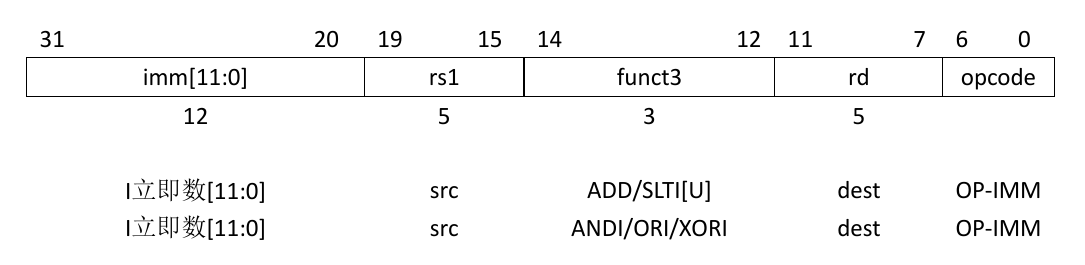
\includegraphics[width=0.8\linewidth]{addi}
		\end{center}
		在取指阶段,这条指令从Instruction Cache中被取出,进入到IR中。
		
		接下来是译码过程,这一步包括取源操作数rs1。它在15--19位,这段地址输入General Register File的Addr1,得到Reg1,进入OP1寄存器。另外,还要处理第20--31位的立即数。将7--31位送入Immediate Extend模块,该模块译出六种不同格式下的立即数,进行符号扩展。在这里,我认为需要补充一个``立即数格式选择器'',以从按照六种式解码得到的的立即数中选择需要的那个。
		\begin{center}
		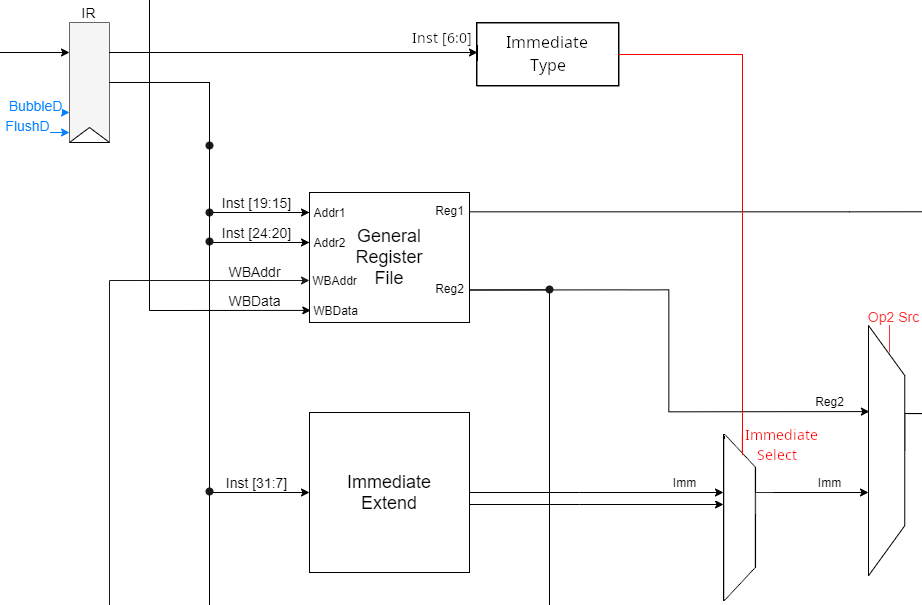
\includegraphics[width=0.8\linewidth]{imm_select_patch}
		\end{center}
		随后,Op2 Src控制信号选择立即数,进入OP2寄存器。
		
		然后是执行过程。控制器根据指令类型,发出ALU Func信号,指导ALU完成对两个操作数寄存器中取出的数进行相加,得到的结果进入RS1寄存器。
		
		在访存阶段,RS1寄存器中的值经过选择器,到达WBData寄存器。
		
		最后是写回阶段,WBData寄存器中的值作为Data Cache的WBData,而在译码阶段得到的目标寄存器的地址,保存在各段的Addr寄存器中,终于来到Data Cache的WBAddr,Data Cache依照这两个信号完成指令运算结果的写回。
		
		\item 间接跳转指令JALR使用I类编码:
		\begin{center}
		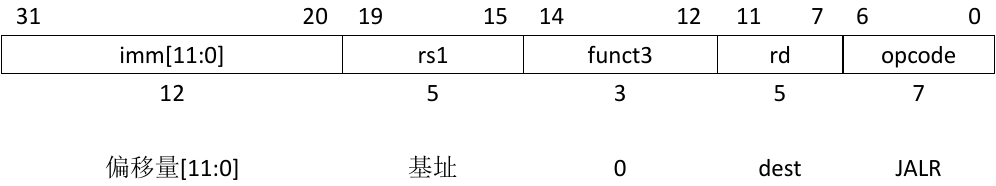
\includegraphics[width=0.8\linewidth]{jalr}
		\end{center}
		在取指与译码阶段,与ADDI基本相同,区别从执行阶段开始。执行阶段主要进行两个运算:一是将跳转指令后面的指令,也就是$\text{pc}+4$,保存到rd中;二是将立即数与rs1相加,最低位设置为0,作为目标地址。在ALU中,完成目标地址的计算,结果通过Jalr Target进入NPC Generator,由Jalr控制信号选择,进入到IF PC寄存器。同时,Load NPC信号控制选择器,使得$\text{PCE}+4$进入到RS1寄存器。
		
		在写回阶段,RS1寄存器中的值写回Data Cache中。
		
		\item Load指令还是I类编码:
		\begin{center}
		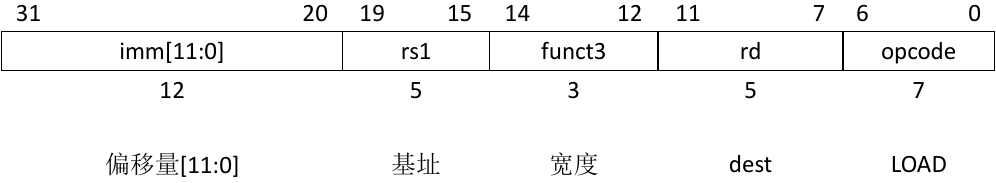
\includegraphics[width=0.8\linewidth]{load}
		\end{center}
		取指与译码依旧与其它I类编码指令相差无几,在执行阶段,ALU把寄存器中取出的数,与经过符号扩展的立即数,相加之后得到了要送往Data Cache的地址Addr。
		\begin{center}
		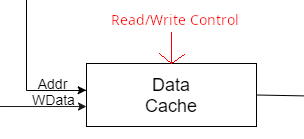
\includegraphics[scale=0.5]{data_cache_control_patch}
		\end{center}
		在访存阶段,控制信号发送到Data Cache,从中读取的数值,再进行数据扩展,需要添加控制信号,以控制Data Cache究竟是进行读操作,还是写操作。扩展器接受到控制信号Load TypeM,不需要做什么改变,结果进入到了选择器。控制信号控制选择器选择从Data Cache中读取到的值,进入了WBData寄存器,准备写回。
		
		写回阶段与其它指令比较类似。
		\item 首先来看一下CSR指令的格式:
		\begin{center}
		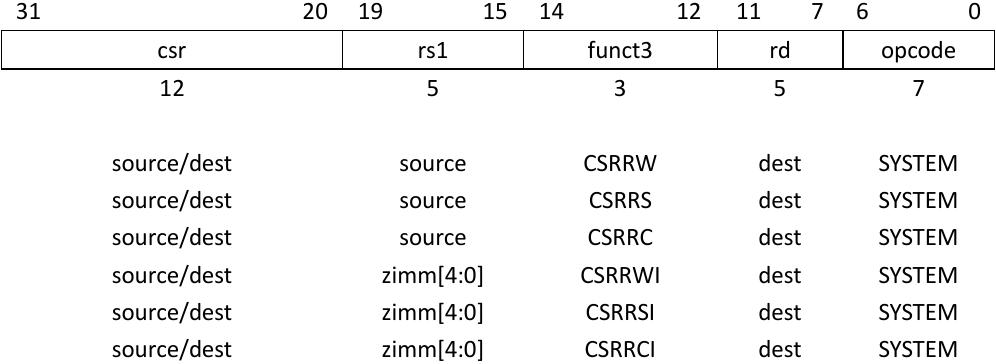
\includegraphics[width=0.8\linewidth]{csr}
		\end{center}
		将其与I类编码指令进行对比,发现两者格式基本相同,因此可以使用相同的译码器。为了简化实现,在译码阶段进行CSR寄存器的读取,在写回阶段进行CSR寄存器的写入。首先,我们需要有寄存器来记录当前的特权级。在译码阶段,根据当前的特权级得知当前指令是否应该被执行。如果正常,则根据计算出来的地址,访问CSR寄存器,读取出其中的值。在执行阶段,根据rs1中的值,或者立即数,计算出要填写到CSR寄存器中的新值。在写回阶段,将CSR寄存器中原来的值写入到rd。由此我们可以看到,需要增加的部件有:CSR寄存器;数据通路有:CSR寄存器到rd,以及计算结果到CSR寄存器。
		
		依次添加这些部件:
		\begin{center}
		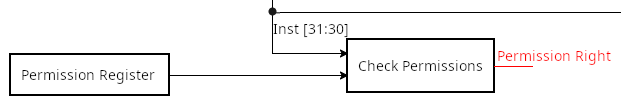
\includegraphics[width=0.8\linewidth]{csr_file_patch}
		\end{center}
		检查权限,如果程序执行了超出当前权限的指令,会体现在控制信号上。
		\begin{center}
		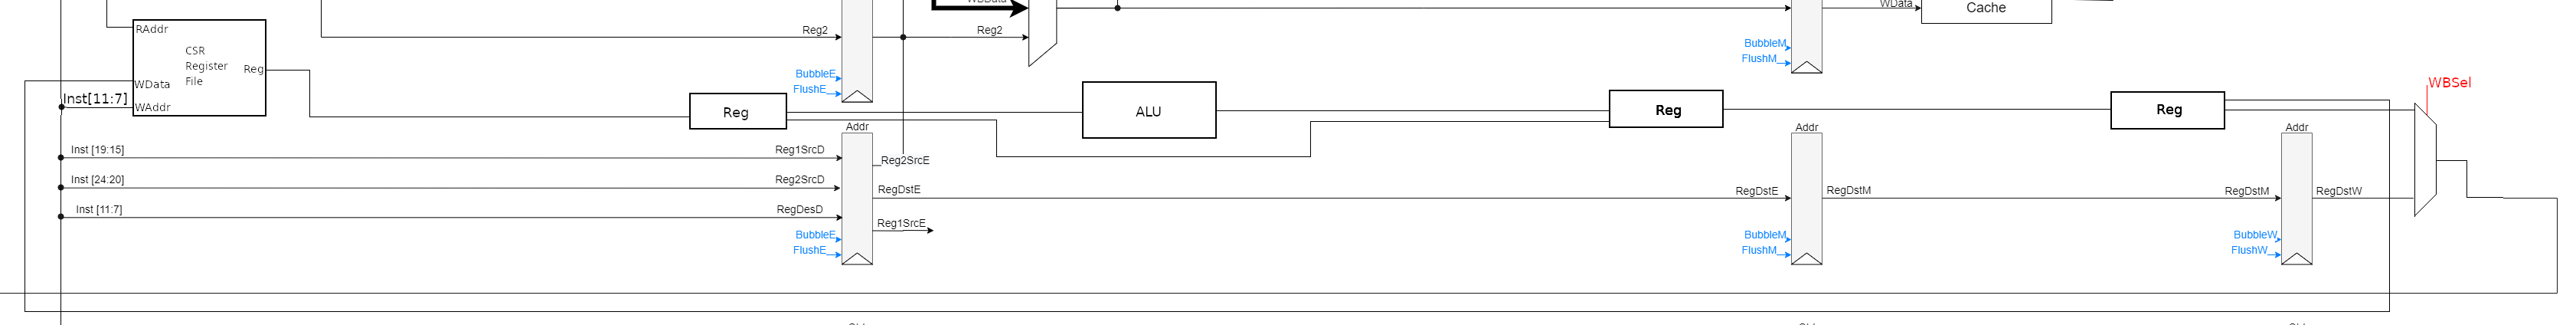
\includegraphics[width=1\linewidth]{csr_full_patch}
		\end{center}
		这部分展示的是添加的电路,用于完成计算,并写入CSR寄存器以及rd寄存器。之所以使用额外的ALU,是因为这部分需要进行的计算与用户级的指令不太一样。
		
		\item 使用五类立即数的指令分别有:
		\begin{enumerate}
		\item[I-type] LW
		\item[J-type] JAL
		\item[S-type] SB
		\item[B-type] BEQ
		\item[U-type] AUIPC
		\end{enumerate}
		拓展过程分为两种情况:符号扩展和0扩展,符号扩展在缺失的位数添加与Inst[31]相同的位,而0扩展则直接添加0。依照我的想法,可以并行生成各种立即数扩展的结果,再根据指令编码类型选择合适的一种。
		
		\item 访问Data Cache的时候,将低2位置0,取出的数值进入Data Extension模块,根据地址的低2位,进行移位,就完成了非对齐的存取。
		
		\item 默认是有符号数。
		
		\item 前面分析过的JALR指令会使Load NPC$=1$,以选择下一条指令的地址。
		
		\item 有优先级,优先处理JAL和JALR,最后才选择PC$+4$。
		
		\item 由于有完整旁路,所以数据相关不需要插入气泡。当遇到分支跳转时,首先需要插入一个气泡,如果预测失误,还需要插入另一个气泡。
		
		\item 在遇到分支跳转的时候,进行Flush;当分支预测失败的时候,也要进行Flush。
		
		\item 没有影响,如果目的操作数是寄存器0,那么无论计算结果是多少,都会被舍弃。当目的操作数为0时,不会从旁路转发,所以没有影响。
	\end{enumerate}
\end{document}